% Cole Nielsen niels538@umn.edu
% EE 2002 Spring 2015
% Formal Lab Report 3

%----------------------------------------------------------------------------------------
%	PACKAGES AND DOCUMENT CONFIGURATIONS
%----------------------------------------------------------------------------------------

\documentclass[12pt]{article}
\usepackage{cmbright}
\usepackage[T1]{fontenc}
\usepackage{circuitikz}
\usepackage{epsfig}
\usepackage{graphicx}
\usepackage{subcaption}
\usepackage[top=1in, bottom= 1in, left=1in, right= 1in]{geometry}
\setlength\parindent{0pt}
\usepackage{fancyhdr}
\pagestyle{fancy}
\usepackage{textcomp}
\usepackage{tikz}
\usepackage{siunitx}
\usepackage{placeins}
\usepackage{titlesec}
\usepackage{cancel} 
\usepackage{tikz}
\usetikzlibrary{shapes.geometric, arrows}
\tikzstyle{box} = [rectangle, rounded corners, minimum width = 3cm, minimum height = 1cm, text centered, draw = black]
\tikzstyle{arrow} = [thick,->,>=stealth]
\usepackage{placeins}

\usepackage{listings}
\usepackage{color}

\definecolor{dkgreen}{rgb}{0,0.6,0}
\definecolor{gray}{rgb}{0.5,0.5,0.5}
\definecolor{mauve}{rgb}{0.58,0,0.82}

\lstset{frame=tb,
  language=,
  aboveskip=3mm,
  belowskip=3mm,
  showstringspaces=false,
  columns=flexible,
  basicstyle={\small\ttfamily},
  numbers=none,
  numberstyle=\tiny\color{gray},
  keywordstyle=\color{blue},
  commentstyle=\color{dkgreen},
  stringstyle=\color{mauve},
  breaklines=true,
  breakatwhitespace=true,
  tabsize=3
}

%----------------------------------------------------------------------------------------
%	DOCUMENT INFORMATION
%----------------------------------------------------------------------------------------

\title{Lab 4 Report\\ \vspace{0.3 in} EE 4111}

\newcommand{\mymeter}[2]{   	% #1 = name , #2 = rotation angle
 \begin{scope}[transform shape,rotate=#2]
   \draw[thick] (#1)node(){$\mathbf V$} circle (11pt);
   \draw[rotate=45,-latex] (#1)  +(-17pt,0) --+(17pt,0);
 \end{scope}
}
\author{Cole \textsc{Nielsen}}
\date{Spring 2016}
\begin{document}
\maketitle 
\pagebreak
%---------------------------------------------------------------------------------------
%----------------------------------------------------------------------------------------
%	Introduction
%----------------------------------------------------------------------------------------
\section*{Spice File}
Below is the SPICE netlist file and the schematic of the OP-AMP design used in this lab for the noise simulations. This is the same compensated OP-AMP designed in the previous lab sessions. Noise simulation was augmented in this file by adding a .NOISE SPICE directive to instantiate a noise simulation on parsing the file through HSPICE.
\FloatBarrier
\begin{figure}[h!]
\begin{center}
 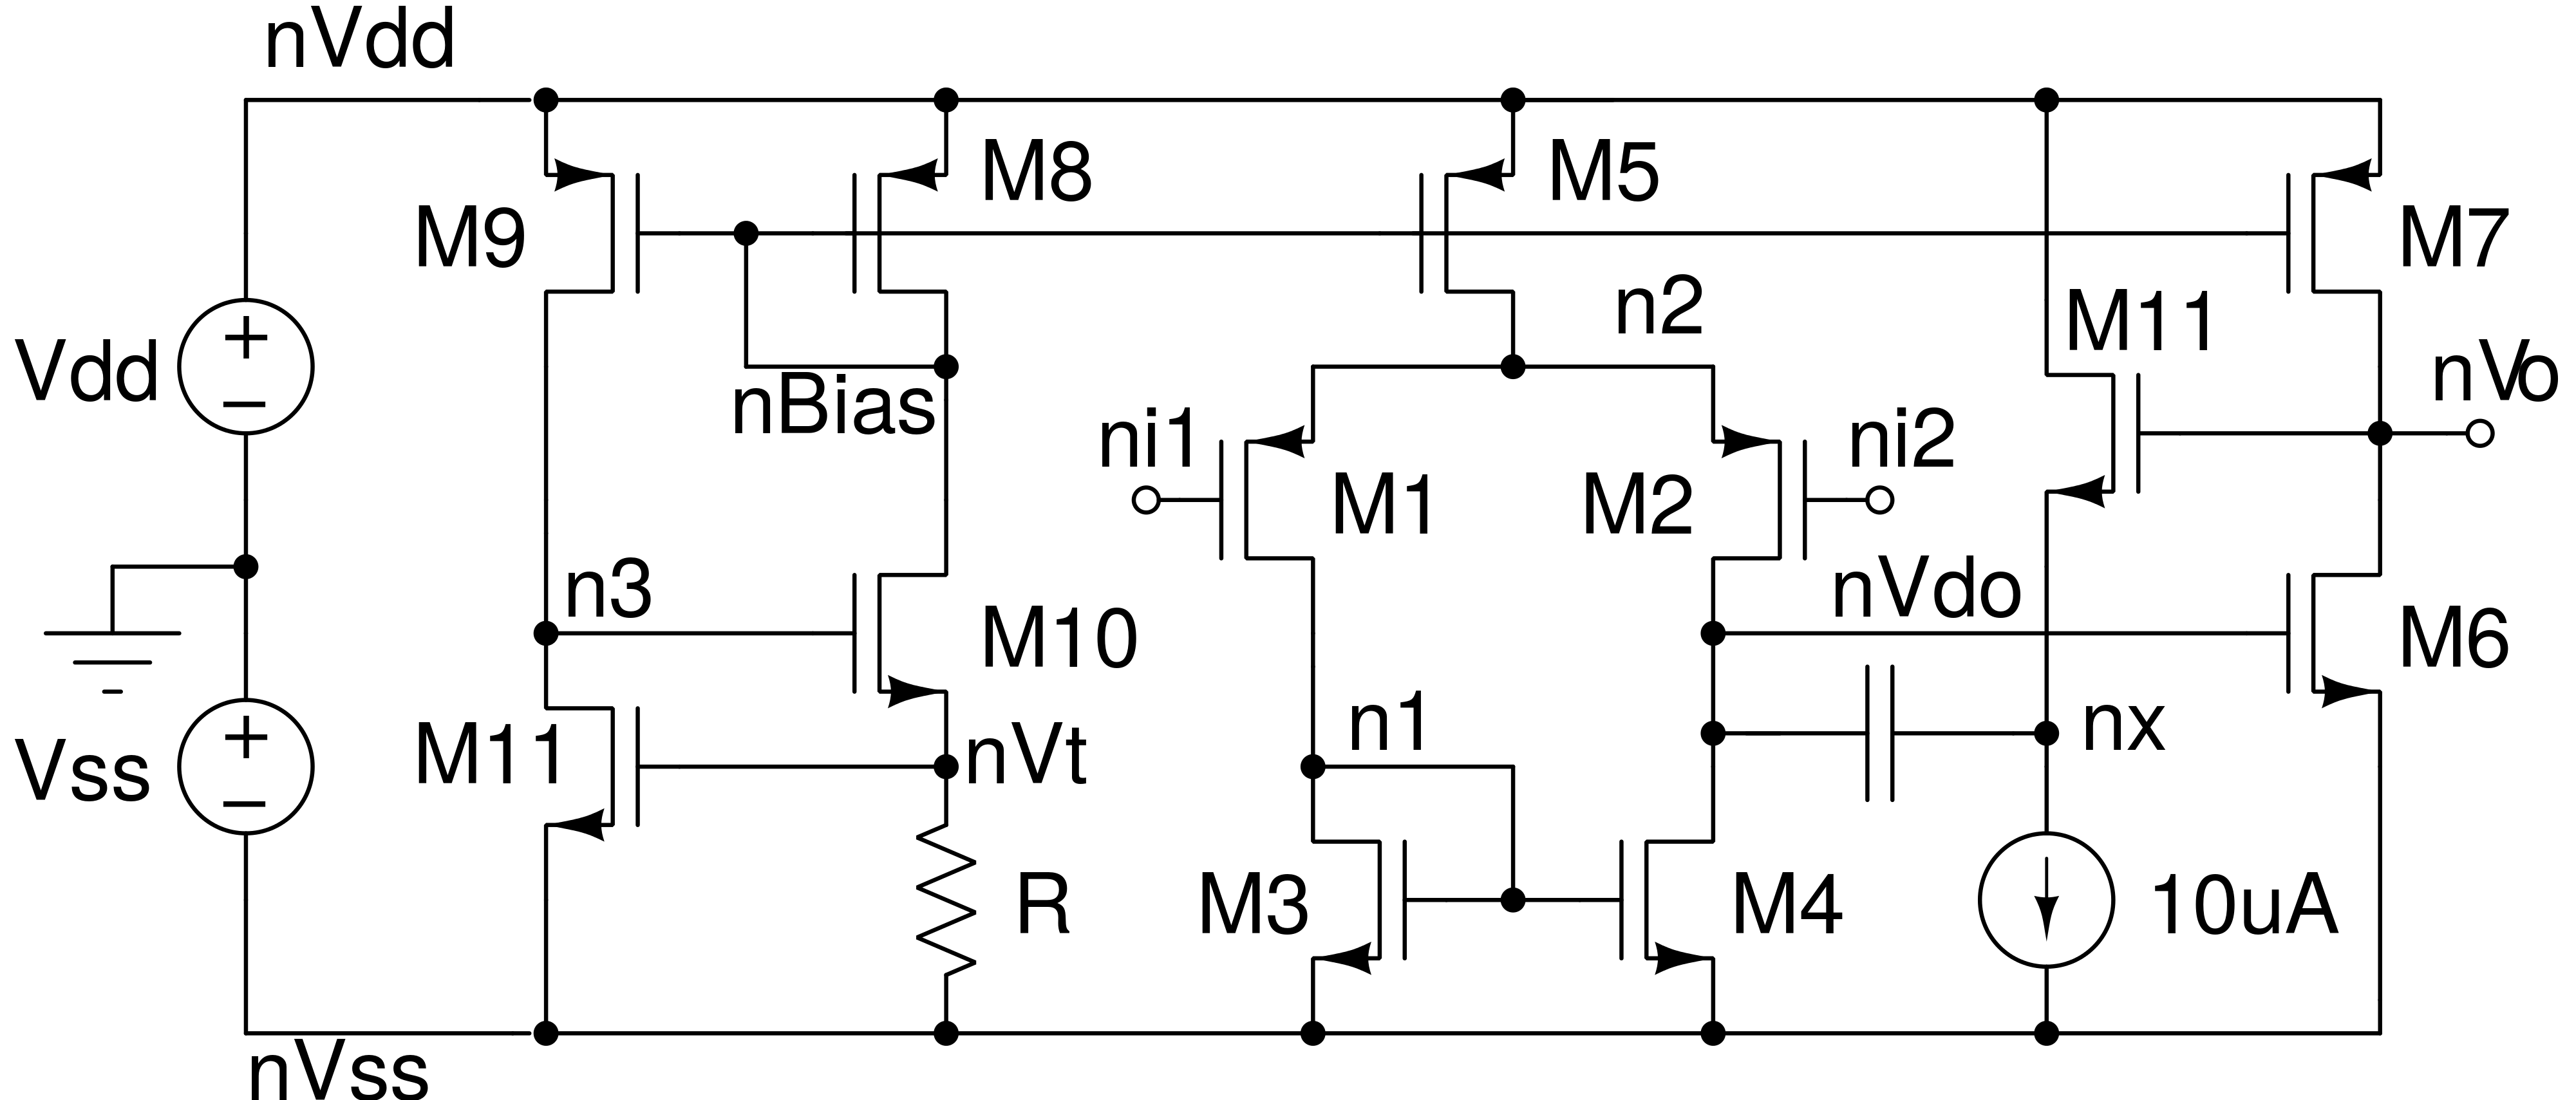
\includegraphics[scale=0.14]{./schem.png}
\end{center}
\end{figure}
\FloatBarrier
\begin{lstlisting}
TWO STAGE OPAMP W/ NOISE SIMULATION
*******SIMULATION PARAMETERS*************
.OPTIONS LIST NODE POST
.AC DEC 100 0.1 1E6
.NOISE V(nvo) Vi2 100

.parameter Vid = 0
.parameter Vic = 0
.parameter Vios = -213.913u ***input offset
.parameter length = 0.25u

***********SUPPLIES*************
Vdd nvdd 0 DC 2V
Vss 0 nvss DC 2V
Vi1 ni1 0 DC Vios
Vi2 ni2 0 DC 0 AC 1 *PULSE(0 1 25n 10p 10p 50n 1u)
*Ei1 ni1 0 VOL = 'Vios + Vic + Vid'
*Ei2 ni2 0 VOL = 'Vic - Vid'

***********CURRENT REF**********
Rb nvt nvss 26000

M8 nbias nbias nvdd nvdd CMOSP W = 30u L = length
M9 n3 nbias nvdd nvdd CMOSP W = 16u L = length
M10 nbias n3 nvt nvss CMOSN W = 10u L = length
M11 n3 nvt nvss nvss CMOSN W = 10u L = length
*Mx D G S B CMOSx W = width L = length

************DIFF AMP*************
M1 n1 ni1 n2 nvdd CMOSP W = 10u L = length
M2 nvdo ni2 n2 nvdd CMOSP W = 10u L = length 
M3 n1 n1 nvss nvss CMOSN W = 4u L = length
M4 nvdo n1 nvss nvss CMOSN W = 4u L = length
M5 n2 nbias nvdd nvdd CMOSP W = 16u L = length

*************STAGE 2*************
M6 nvo nvdo nvss nvss CMOSN W = 2.3u L = length
M7 nvo nbias nvdd nvdd CMOSP W =6u L = length
*Cl nvo 0 10p

***********COMPENSATION*************
Cc nvdo nx 0.24pF
M12 nvdd nvo nx nvss CMOSN W = 100u L = length
Ibias nx nvss 10u

.MODEL CMOSN NMOS (
+LEVEL   = 49             acm     = 3              hdif    = 0.35e-6
+VERSION = 3.1            TNOM    = 27             TOX     = 5.7E-9
+XJ      = 1E-7           NCH     = 2.3549E17      VTH0    = 0.4365497
+K1      = 0.3915623      K2      = 0.0175145      K3      = 1E-3
+K3B     = 2.6588343      W0      = 1E-7           NLX     = 1.111465E-7
+DVT0W   = 0              DVT1W   = 0              DVT2W   = 0
+DVT0    = -0.0408321     DVT1    = 0.0746768      DVT2    = 0.307109
+U0      = 407.1177485    UA      = 9.442714E-11   UB      = 1.092986E-18
+UC      = 1.63196E-11    VSAT    = 1.365087E5     A0      = 1.3189329
+AGS     = 0.2711719      B0      = 3.291713E-8    B1      = -1E-7
+KETA    = 4.645753E-3    A1      = 0              A2      = 1
+RDSW    = 439.9558234    PRWG    = 0.0345487      PRWB    = -0.0441065
+WR      = 1              WINT    = 1.645705E-9    LINT    = 1.116516E-9
+XL      = 3E-8           XW      = 0              DWG     = -1.494138E-9
+DWB     = 1.459097E-8    VOFF    = -0.1026054     NFACTOR = 0.1344887
+CIT     = 0              CDSC    = 1.527511E-3    CDSCD   = 0
+CDSCB   = 0              ETA0    = 1.930311E-3    ETAB    = 2.946158E-4
+DSUB    = 0.0214865      PCLM    = 1.3387947      PDIBLC1 = 0.480652
+PDIBLC2 = 9.034986E-3    PDIBLCB = -1E-3          DROUT   = 0.5593223
+PSCBE1  = 9.843289E9     PSCBE2  = 2.10878E-9     PVAG    = 1.0033136
+DELTA   = 0.01           MOBMOD  = 1              PRT     = 0
+UTE     = -1.5           KT1     = -0.11          KT1L    = 0
+KT2     = 0.022          UA1     = 4.31E-9        UB1     = -7.61E-18
+UC1     = -5.6E-11       AT      = 3.3E4          WL      = 0
+WLN     = 1              WW      = -1.22182E-16   WWN     = 1.2127
+WWL     = 0              LL      = 0              LLN     = 1
+LW      = 0              LWN     = 1              LWL     = 0
+CAPMOD  = 2              XPART   = 0.4            CGDO    = 3.11E-10
+CGSO    = 3.11E-10       CGBO    = 1E-11          CJ      = 1.758521E-3
+PB      = 0.99           MJ      = 0.457547       CJSW    = 4.085057E-10
+PBSW    = 0.8507757      MJSW    = 0.3374073      PVTH0   = 7.147521E-5
+PRDSW   = -67.2161633    PK2     = -1.344599E-3   WKETA   = 3.035972E-3
+LKETA   = -9.0406E-3     LAGS    = -0.3012        NLEV = 2	KF	= 1E-26)
*
.MODEL CMOSP PMOS (
+LEVEL   = 49             acm     = 3              hdif    = 0.35e-6
+VERSION = 3.1            TNOM    = 27             TOX     = 5.7E-9
+XJ      = 1E-7           NCH     = 4.1589E17      VTH0    = -0.6586391
+K1      = 0.5199897      K2      = 0.0357513      K3      = 0
+K3B     = 15.5613889     W0      = 1E-6           NLX     = 1E-9
+DVT0W   = 0              DVT1W   = 0              DVT2W   = 0
+DVT0    = 2.6100181      DVT1    = 0.4363142      DVT2    = -0.042436
+U0      = 196.024903     UA      = 2.767112E-9    UB      = 1.90709E-18
+UC      = 6.166867E-11   VSAT    = 1.975064E5     A0      = 0.2398712
+AGS     = 0.0943234      B0      = 3.21184E-6     B1      = 5E-6
+KETA    = 0.0312217      A1      = 0              A2      = 1
+RDSW    = 997.072701     PRWG    = -0.1916111     PRWB    = -0.495
+WR      = 1              WINT    = 2.527293E-9    LINT    = 1.254514E-8
+XL      = 3E-8           XW      = 0              DWG     = -3.253948E-8
+DWB     = 4.92072E-8     VOFF    = -0.15          NFACTOR = 1.5460516
+CIT     = 0              CDSC    = 1.413317E-4    CDSCD   = 0
+CDSCB   = 0              ETA0    = 0.7241245      ETAB    = -0.240523
+DSUB    = 1.0813613      PCLM    = 2.0772083      PDIBLC1 = 4.31459E-4
+PDIBLC2 = 0.0252121      PDIBLCB = -9.960722E-4   DROUT   = 0.0432774
+PSCBE1  = 3.191047E10    PSCBE2  = 1.323218E-8    PVAG    = 0.0420525
+DELTA   = 0.01           MOBMOD  = 1              PRT     = 0
+UTE     = -1.5           KT1     = -0.11          KT1L    = 0
+KT2     = 0.022          UA1     = 4.31E-9        UB1     = -7.61E-18
+UC1     = -5.6E-11       AT      = 3.3E4          WL      = 0
+WLN     = 1              WW      = 0              WWN     = 1
+WWL     = 0              LL      = 0              LLN     = 1
+LW      = 0              LWN     = 1              LWL     = 0
+CAPMOD  = 2              XPART   = 0.4            CGDO    = 2.68E-10
+CGSO    = 2.68E-10       CGBO    = 1E-11          CJ      = 1.902493E-3
+PB      = 0.9810285      MJ      = 0.4644362      CJSW    = 3.142741E-10
+PBSW    = 0.9048624      MJSW    = 0.3304452      PVTH0   = 4.952976E-3
+PRDSW   = 29.8169373     PK2     = 3.383373E-3    WKETA   = -7.913501E-3
+LKETA   = -0.0208318     NLEV	= 2	KF	= 1E-26)
*
.end
\end{lstlisting}
\section{Basic OP-AMP Noise Analysis}
The first objective of this lab was to analyze the output noise of the compensated OPAMP designed in the previous labs. This first set of simulations only factored in simple thermal (Johnson-Nyquist) noise, which is generated by all the resistors and MOSFETs of the circuit. Thermal noise is quantified by the following relation:
\begin{equation}
\overline{v_n^2} = 4k_bTR
\end{equation}
Where $\overline{v_n^2}$ is the thermal noise variance, $k_b$ is Boltzmann's constant, T is the absolute temperature given in Kelvin and R is the resistance of the noise generating medium. This relation tells us one important detail: thermal noise is dependent on the resistance of the devices for this simulation, as the temperature is assumed to be constant. Therefore, the resistors and MOSFETs of the circuit will exhibit thermal noise (the MOSFETs are resistive primarily due to their resistive channels). The noise analysis was performed in SPICE by adding a .NOISE statement that simulates noise for the ouput node nVo relative to an input source, for this simulation ni2 was used. The OP-AMP was simulated in an open-loop configuration with the other input ni1 connected to ground (with input offset correction included). The noise simulation was set to simulate for 0.1 Hz to 100 MHz in the .AC statement. The results of this simulation are presented below:

\FloatBarrier
\begin{figure}[h!]
\begin{center}
 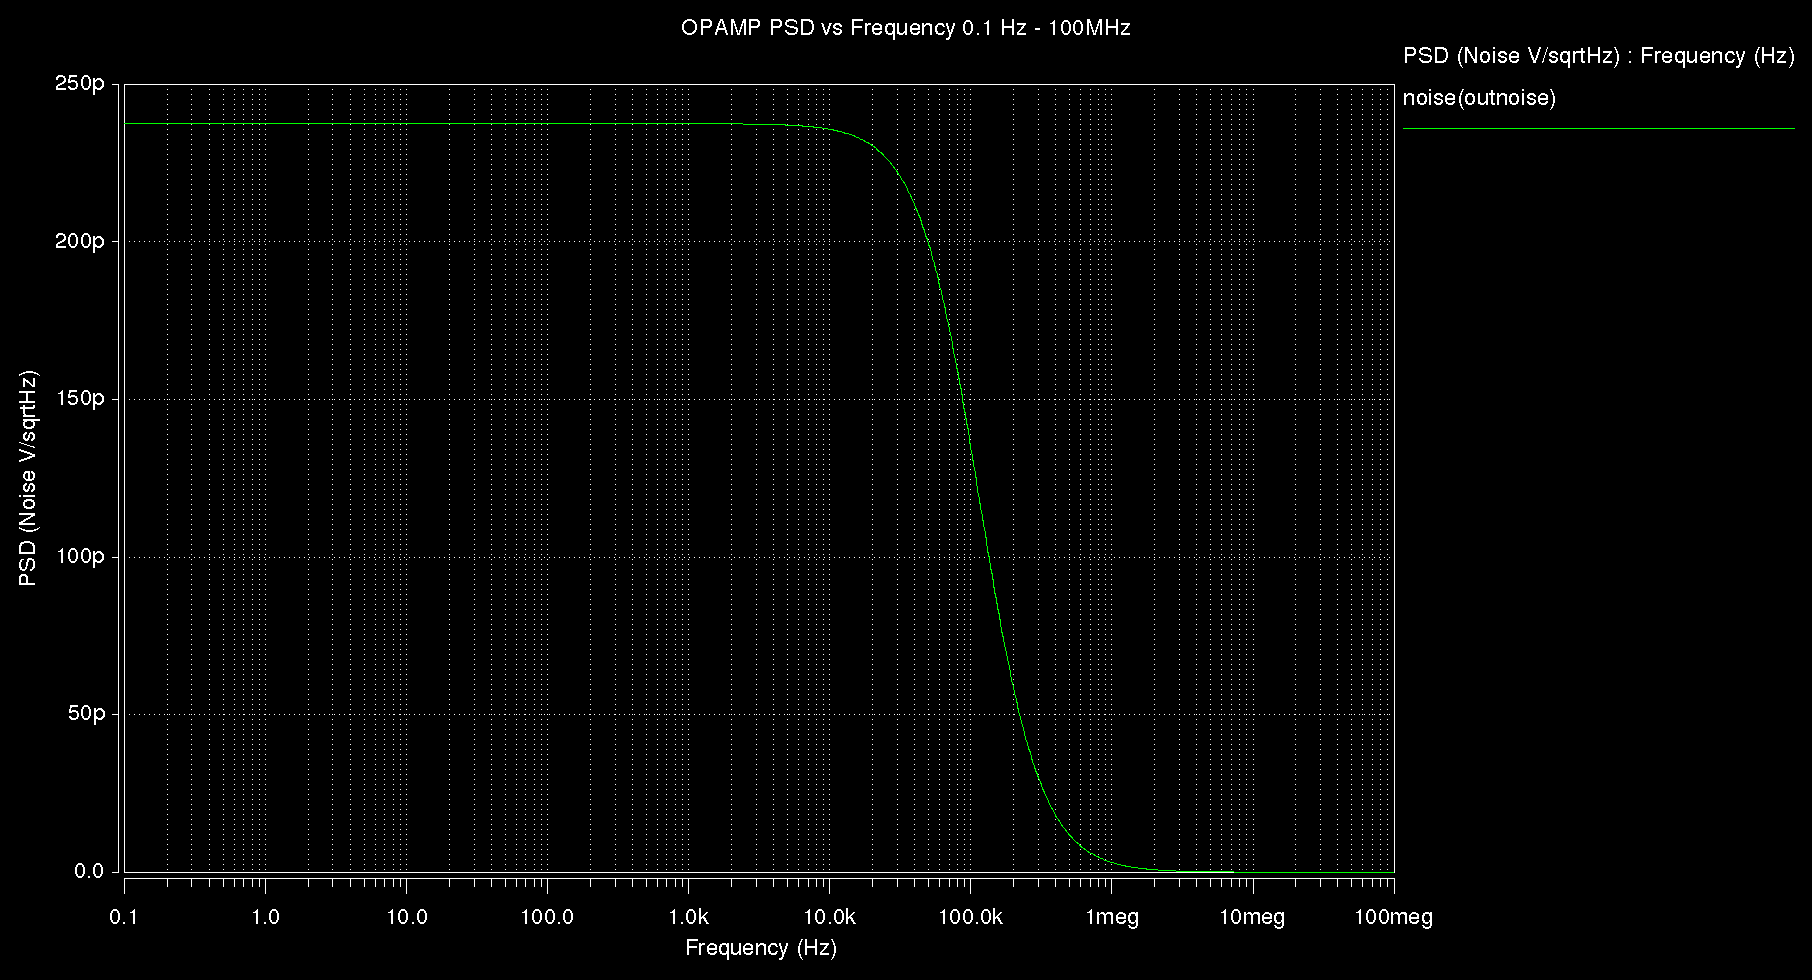
\includegraphics[scale=0.23]{./noise1a.png}
\end{center}
\end{figure}
\FloatBarrier
This plot gives total noise power spectral density of the output relative to the OPAMP input in units of $\frac{V}{\sqrt{Hz}}$, which is just the square root of the noise variance given in equation 1. It can be seen that the noise begins to drop off after approximately 10kHz, due to the pole location of the OP-AMP compensation. The shape of the response is effectively the transfer function for the input conpensation as the noise given no poles should follow a uniform distribution, so the only changes for the PSD should be in accordance to the pole of the OP-AMP. Total RMS (root-mean-square) noise of the OP-AMP on the output was determined by integrating the PSD over the simulated frequency range, where the interval of intergration is given by [${f_l}$,${f_h}$]:
\begin{equation}
V_{n,RMS} = \int _{f_l}^{f_h} \sqrt{\overline{v_n^2}}df
\end{equation}
Below is the plot showing the result of this integration. Total RMS Noise on the output was found to be 42.772$\mu$V on the ouput, if no other filtering is used and a bandwidth of 100 MHz is utilized. 
\FloatBarrier
\begin{figure}[h!]
\begin{center}
 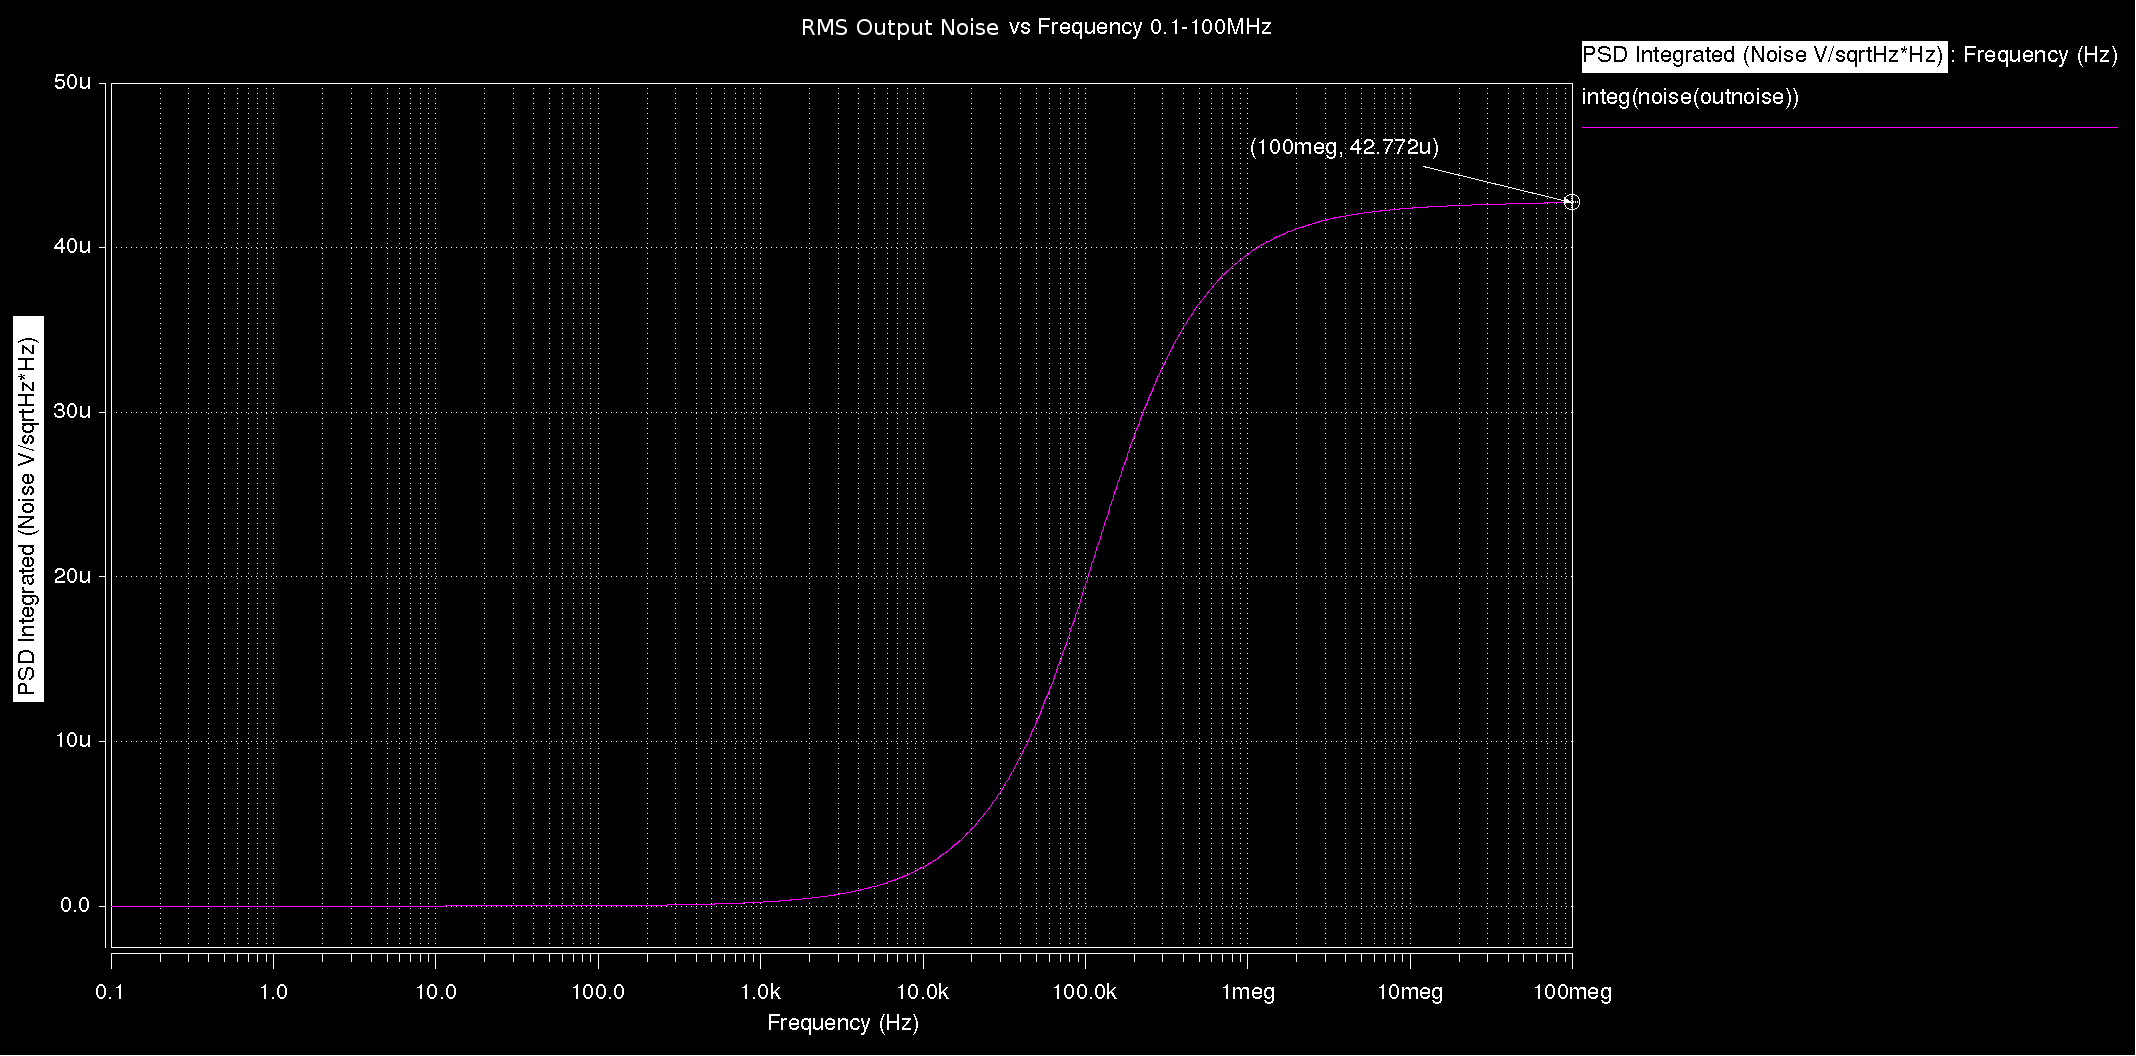
\includegraphics[scale=0.2]{./noise1b.png}
\end{center}
\end{figure}
\FloatBarrier
\section{Flicker Noise Simulation Modification}
The second objective of this lab was to add flicker noise to the simulation for the OP-AMP. The provided mosfet models used in this lab do not factor in flicker ($1/f$) noise, so several parameters had to be added to include it in simulation. The basic model parameters in LEVEL 49 are NLEV, which is the noise equation selector, AF, the flicker noise exponent, and KF which is the flicker noise coefficient. NLEV was set to the default value of 2, therefore the standard noise simulation equations were used. AF and KF are parameters of the following flicker noise equation:
\begin{equation}
\overline{i_n^2} = \textnormal{KF} \frac{I}{f^\textnormal{AF}}
\end{equation}
Where $\overline{i_n^2}$ is the flicker noise PSD for current (SPICE simulates in terms of current). The equivalent PSD in terms of voltage can be found by multiplying the current PSD by R$^2$. Notice the flicker noise is directly proportional to DC current through an element, and inversely to the frequency. An important implication of this is the flicker noise decreases with frequency, eventually falling below the thermal noise. The intersection point of flicker noise is the transisition frequency. It should be noted because of this, flicker noise dominates at low frequencies. This effect is illustrated below (where $f_a$ is the intersection frequency).

\FloatBarrier
\begin{figure}[h!]
\begin{center}
 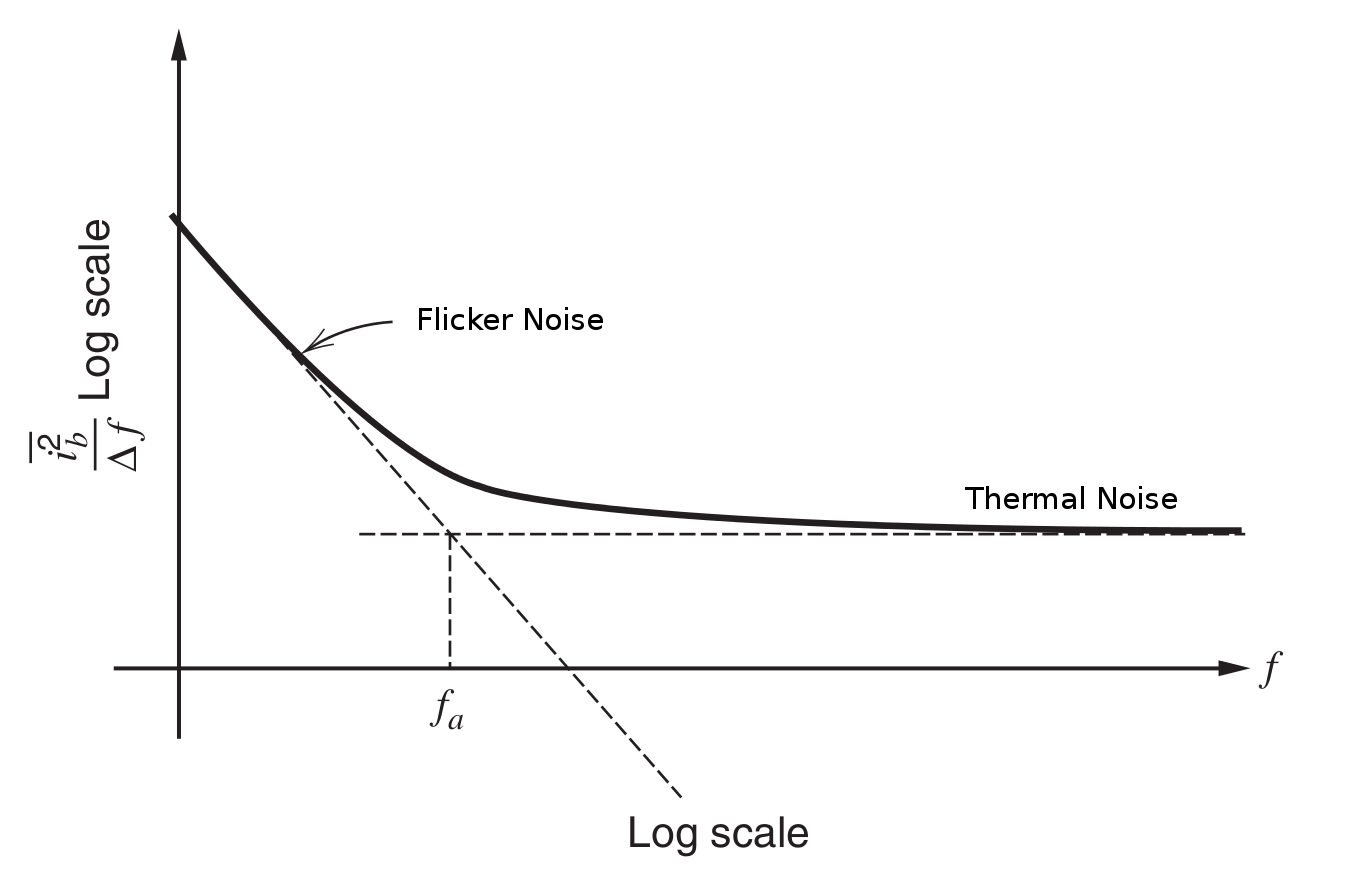
\includegraphics[scale=0.2]{./flick.png}
\end{center}
\end{figure}
\FloatBarrier
The values for KF was adjusted until the transition frequency between the two noise curves was approximately 10kHz, which is typical for MOSFETs. This value was found to be KF = 1E-26 for AF = 1. The PSD for output noise of the OPAMP including this flicker noise is shown below:
\FloatBarrier
\begin{figure}[h!]
\begin{center}
 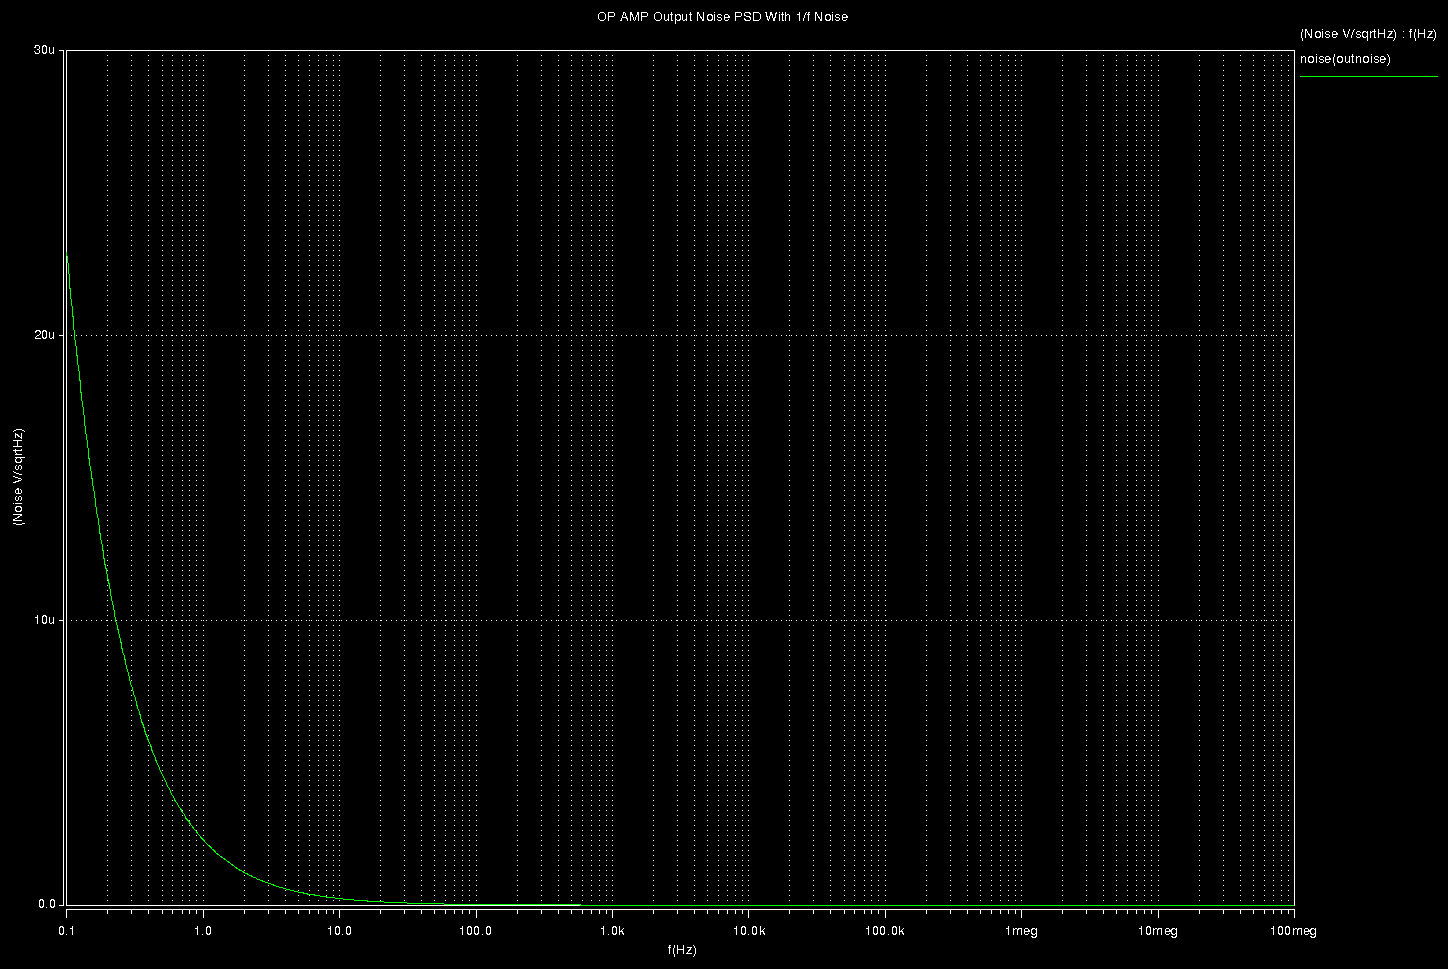
\includegraphics[scale=0.3]{./psd_flicker.png}
\end{center}
\end{figure}
\FloatBarrier
The total RMS noise on the output can be calculated by again integrating the PSD over the simulated frequency range, using the calculation tools built into COSMOSCOPE. Total RMS noise over the whole band analyzed was calculated to be approximately 67$\mu$V, larger than the approximately 42$\mu$V seen without inclusion of flicker noise. Looking at the integrated PSD, the two regions where flicker noise is dominant and then where thermal noise is dominant can be observed. The flicker noise region is the first flat line, and the thermal noise region is where the slope suddenly chages near 20kHz and then eventually tapers off due to the OP-AMP's compensation bringing the gain to essentially 0. 
\FloatBarrier
\begin{figure}[h!]
\begin{center}
 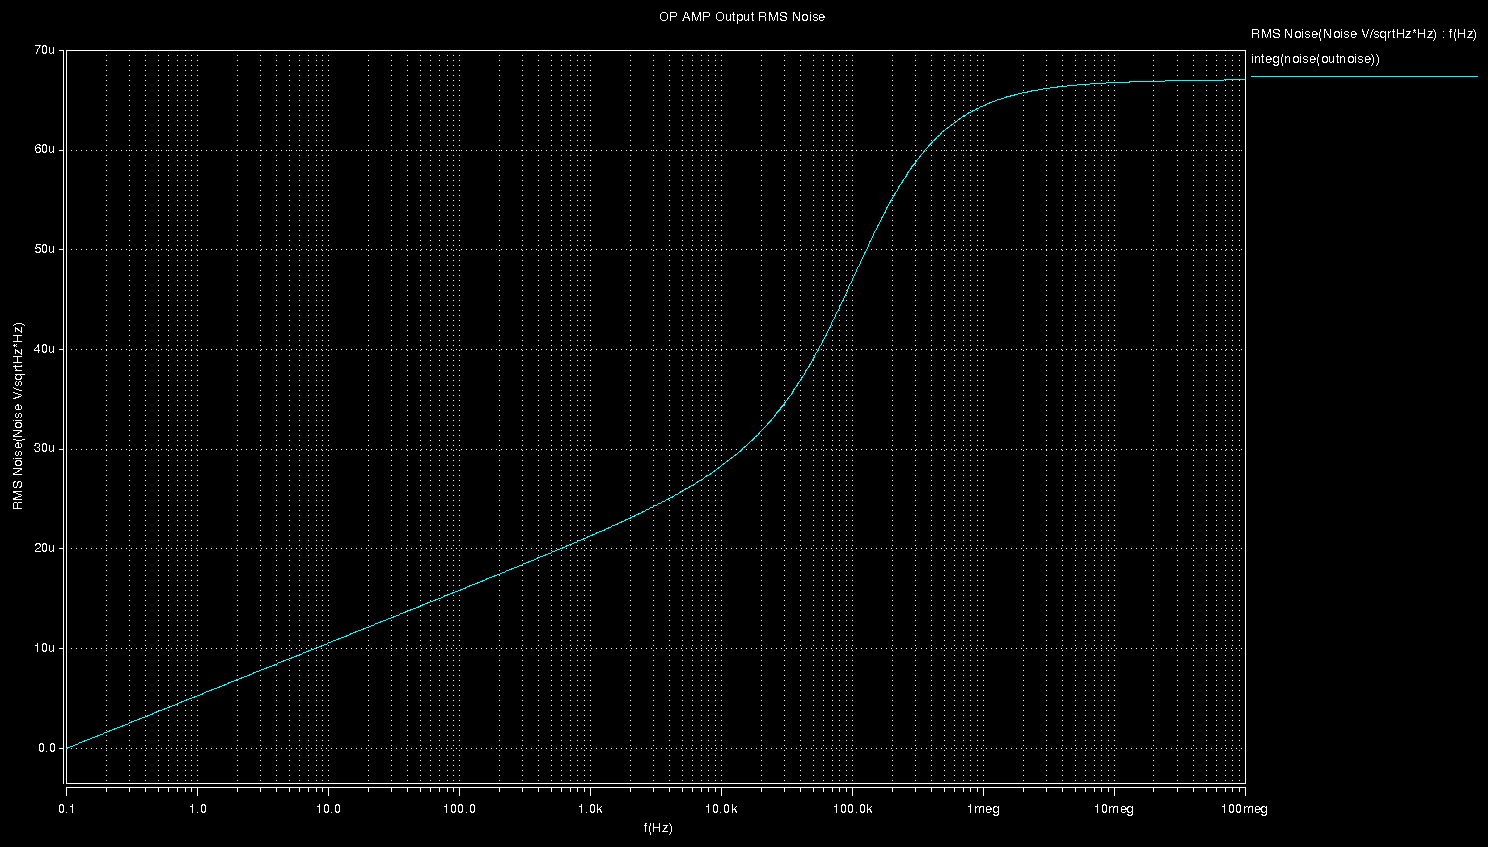
\includegraphics[scale=0.3]{./out_noise_flick.png}
\end{center}
\end{figure}
\FloatBarrier
\section{Input Referred Noise}
The objective of this part of the lab was to find the equivalent referred input noise PSD for the OP-AMP design. Equivalent input referred noise is simply the noise that would be fed into the input of a noiseless OP-AMP in order to get the same output noise of that OP-AMP if it was noisy with no input signal. This is illustrated below, where $\overline{v_{n,i}^2}$ is the input referred noise variance and $\overline{v_{n}^2}$ is the measured output noise variance:
\FloatBarrier
\begin{figure}[h!]
  \begin{center}
    	\hspace*{0.5in}\resizebox{0.9\textwidth}{!}{% XCircuit output "noisea.tex" for LaTeX input from noisea.eps
\def\putbox#1#2#3#4{\makebox[0in][l]{\makebox[#1][l]{}\raisebox{\baselineskip}[0in][0in]{\raisebox{#2}[0in][0in]{\scalebox{#3}{#4}}}}}
\def\rightbox#1{\makebox[0in][r]{#1}}
\def\centbox#1{\makebox[0in]{#1}}
\def\topbox#1{\raisebox{-0.60\baselineskip}[0in][0in]{#1}}
\def\midbox#1{\raisebox{-0.20\baselineskip}[0in][0in]{#1}}
   \scalebox{1}{
   \normalsize
   \parbox{7.58333in}{
   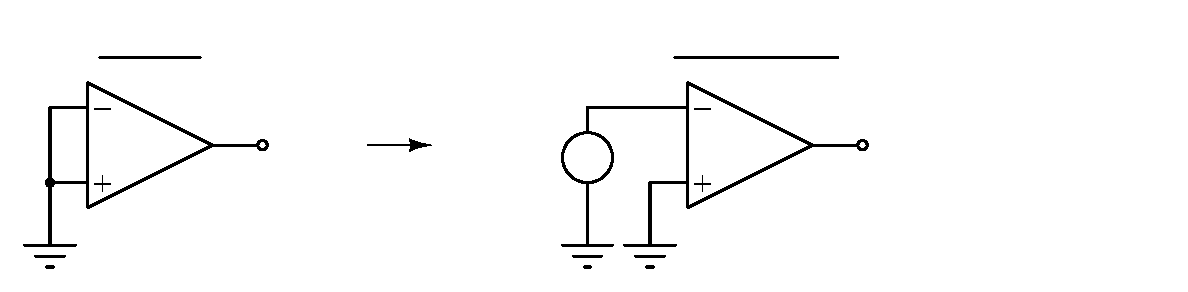
\includegraphics[scale=1]{noisea}\\
   % translate x=496 y=348 scale 0.38
   \putbox{1.81in}{0.79in}{1.20}{$\overline{V_{n}}^2$}%
   \putbox{3.06in}{0.70in}{1.20}{$\overline{V_{n,i}}^2$}%
   \putbox{5.72in}{0.79in}{1.20}{$\overline{V_{n}}^2$}%
   \putbox{0.64in}{1.54in}{1.20}{Noisy}%
   \putbox{4.47in}{1.54in}{1.20}{Noiseless}%
   } % close 'parbox'
   } % close 'scalebox'
   \vspace{-\baselineskip} % this is not necessary, but looks better
}
  \end	{center}
 % \caption{NaCl freezing point depression versus molality}
\end {figure}
\FloatBarrier
The noise can simply be found by finding the output noise in a closed-loop follower configuration $\overline{v_{n,loop}^2}$, and then by finding the voltage transfer function for the follower, $|H(f)|$. Input refered noise is then given by the following relation for the previously mentioned quanities:
\begin{equation}
\overline{v_{n,i}^2} = \frac{\overline{v_{n,loop}^2}}{|H(f)|}
\end{equation}
The circuits used for this are shown below:

\FloatBarrier
\begin{figure}[h!]
  \begin{center}
    	\hspace*{0.5in}\resizebox{0.9\textwidth}{!}{% XCircuit output "lab4n.tex" for LaTeX input from lab4n.eps
\def\putbox#1#2#3#4{\makebox[0in][l]{\makebox[#1][l]{}\raisebox{\baselineskip}[0in][0in]{\raisebox{#2}[0in][0in]{\scalebox{#3}{#4}}}}}
\def\rightbox#1{\makebox[0in][r]{#1}}
\def\centbox#1{\makebox[0in]{#1}}
\def\topbox#1{\raisebox{-0.60\baselineskip}[0in][0in]{#1}}
\def\midbox#1{\raisebox{-0.20\baselineskip}[0in][0in]{#1}}
   \scalebox{1.08333}{
   \normalsize
   \parbox{7.45312in}{
   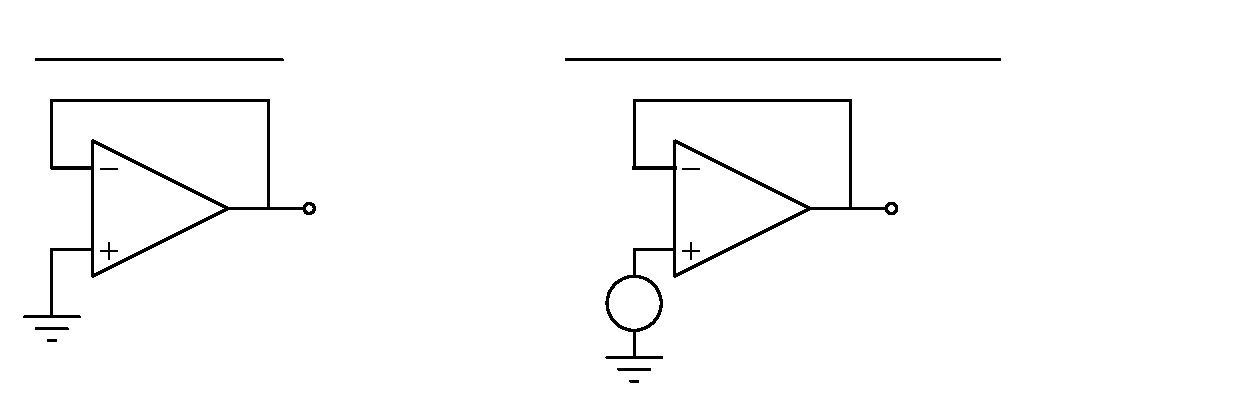
\includegraphics[scale=0.923077]{lab4n}\\
   % translate x=865 y=381 scale 0.41
   \putbox{0.22in}{2.11in}{1.20}{Follower Noise}%
   \putbox{3.47in}{2.11in}{1.20}{Follower Transfer Function}%
   \putbox{3.13in}{0.36in}{1.20}{AC 1}%
   \putbox{1.88in}{1.03in}{1.20}{$\overline{V_{o,loop}}^2$}%
   \putbox{5.47in}{1.03in}{1.20}{$V_o(f)$}%
   \putbox{4.63in}{0.45in}{1.20}{$|H(f)| = \frac{V_o(f)}{V_i(f)}$}%
   \putbox{3.13in}{0.61in}{1.20}{$V_i(f)$}%
   } % close 'parbox'
   } % close 'scalebox'
   \vspace{-\baselineskip} % this is not necessary, but looks better
}
  \end	{center}
 % \caption{NaCl freezing point depression versus molality}
\end {figure}
\FloatBarrier

This works because the closed loop noise should be the input referred noise corrupted by the transfer characteristics of the follower. The transfer characteristics of the follower can simply be found, as done, using a AC analysis of the follower in terms of output to input voltage. The effects of the follower transfer characteristics on the observed output noise can easily be cancelled by just dividing the output observed noise by the follower transfer characteristic. Below is the simulation result, showing the input referred noise on top and the output noise and follower characteristic below. The flicker noise can be seen as the downward sloped line, appearing linear due to the log scaling. The thermal noise can be seen as the horizontal region after approximately 9.2kHz. It should be noted that the thermal noise dominates the flicker noise after 9.2kHz (the noise transition frequency), as the thermal noise is always of constant power, where as the flicker noise decreases as $\frac{1}{f}$, shrinking so small as $f$ increases that only thermal noise is visible.
\FloatBarrier
\begin{figure}[h!]
\begin{center}
 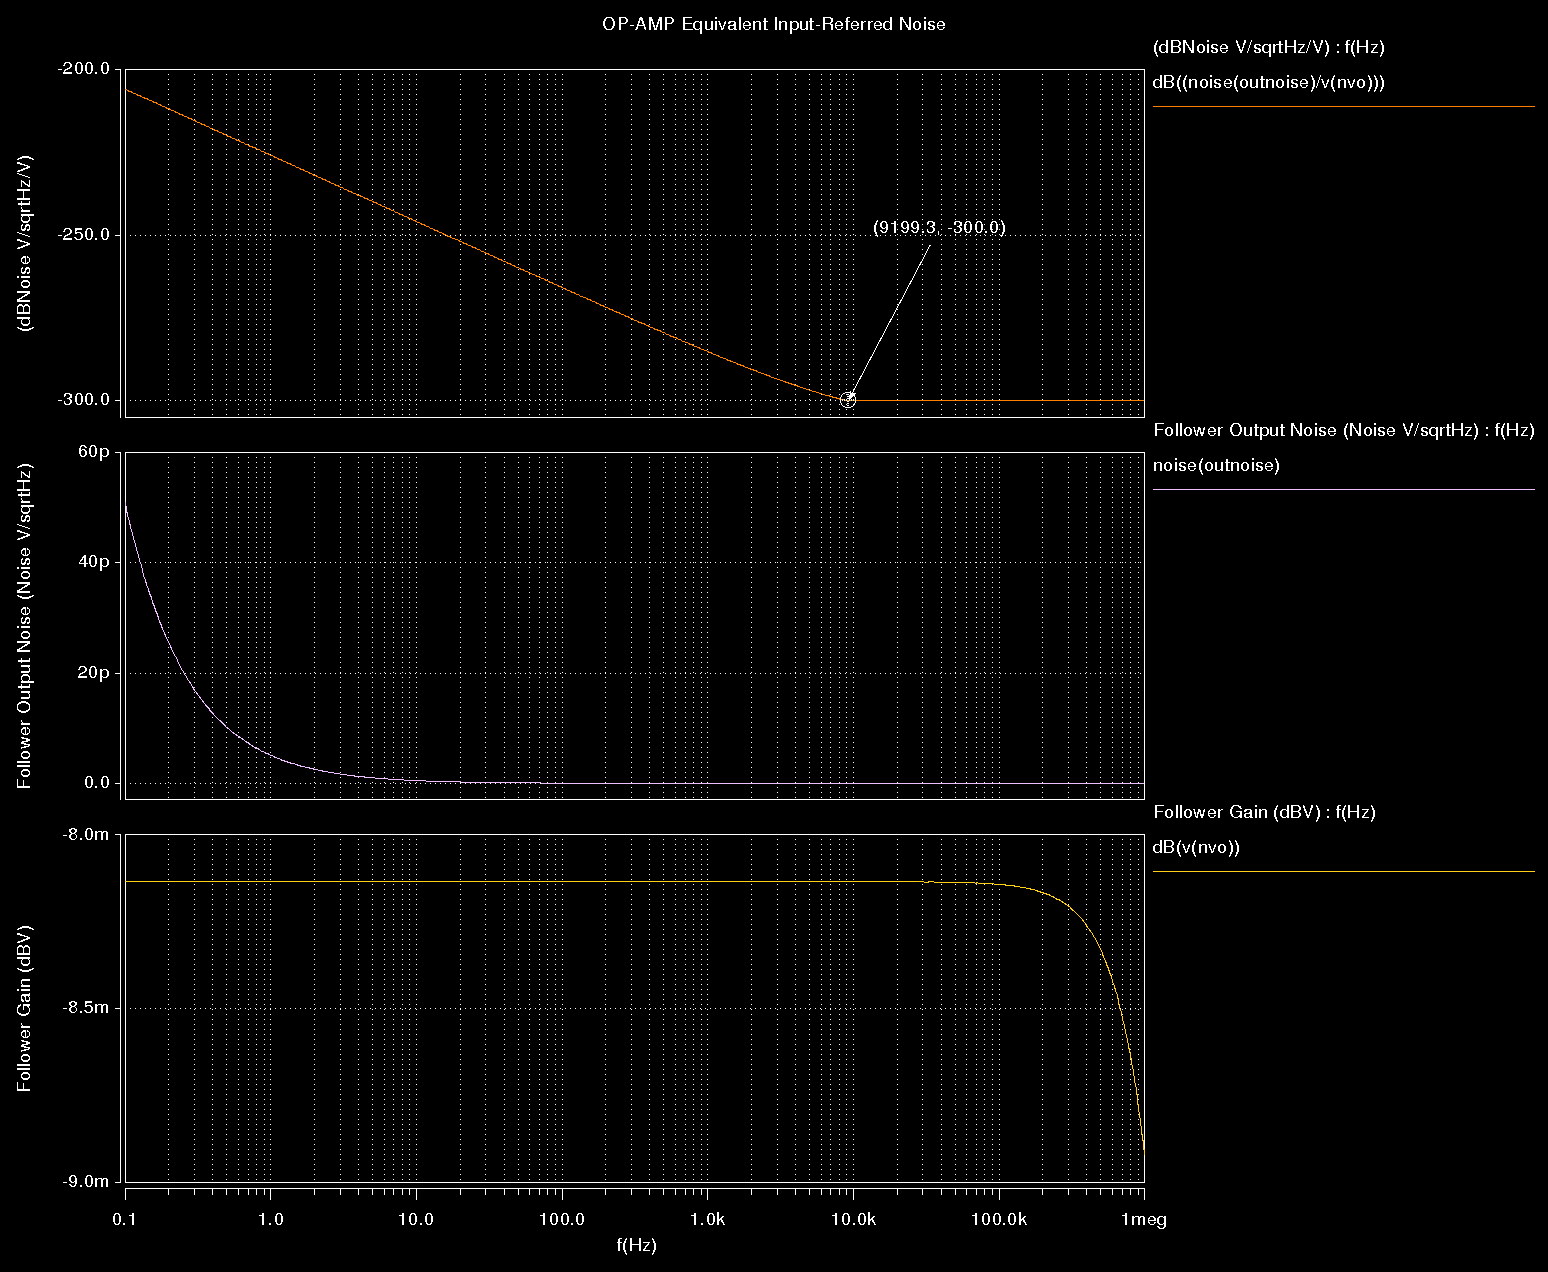
\includegraphics[scale=0.3]{./ref_noise.png}
\end{center}
\end{figure}
\FloatBarrier

\end{document}
